\section{Finite Volume Method for Elliptic PDEs}
\numericsubsection{FVM for Poisson Problems (Voronoi)}
\begin{addmargin}[1em]{0em}
    {\color{teal}
        Divergence Theorem: Given a vector field $\vec{f}(x,y)$.
        The flux integral over the boundary $\partial\Gamma$ satisfies:
        \begin{align*}
            \oint_{\partial\Gamma}\vec{f}(x,y)\ d\vec{n} = \int_\Gamma \mathrm{div}(\vec{f}(x,y))\ dA
            \quad(\vec{n} = \text{outer normal vector})
        \end{align*}
    }
\end{addmargin}

Integrating Poisson's equation $\Delta u = f$ over a non-pathological domain $\Gamma\subset\Omega$ leads to
\begin{align*}
    \int_\Gamma \Delta u(x,y)\ dxdy = \int_\Gamma f(x,y)\ dxdy\quad{\color{gray}\text{(f=0 for Laplacian eq.)}}
\end{align*}
by the divergence theorem, this implies

\colorbox{shadecolor}{$
    \displaystyle
    \underbrace{\oint_{\partial\Gamma}\mathrm{grad}(u(x,y))\ d\vec{n}}_\text{Approx. by Voronoi cells}
    = \int_\Gamma f(x,y)\ dxdy
$}

for all non-pathological domains $\Gamma\subset\Omega$.

The \emph{left flux integral} will then be discretised along a finite set of normal derivatives
for a discrete, polygonal cell:
\begin{align*}
    \oint_{\partial\Gamma}\cdots\ d\vec{n} \approx \sum_j = \frac{u(P_j) - u(P_i)}{\delta_{i,j}}\cdot \lambda_{i,j}
\end{align*}
for each normal $j$ of cell $i$ with two cell points $P_i,P_j$ and let
$\delta_{i,j}$ be the distance between the two cell points
and $\lambda_{i,j}$ the length of the common edge of the two cells.

The \emph{right surface integral} needs to be approximated numerically.
Easiest way: take function value at Voronoi point and multiply by cell area
(obviously not a very good approximation). For the Lapace equation, it's just zero.

We therefore receive a system of linear equations $Av=f$ for the cell values.

\paragraph{Discretisation of Geometry: Voronoi Cells}
We can apply the following ``algorithm'':
\begin{enumerate}
    \item Replace curved boundary by some polygonal approximation
    \item Choose $n$ Voronoi points $P_k$ in $\Omega$ and construct for each point its Voronoi cell
    \item Compute points that are nearest to the corresponding edge of the boundary where a cell has no close neighbour
\end{enumerate}

\makebox[\columnwidth]{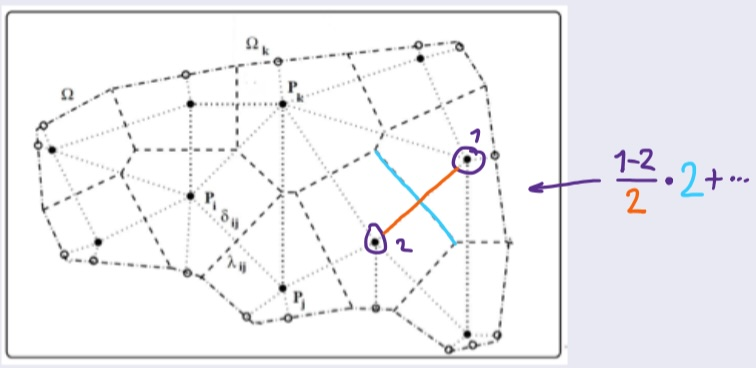
\includegraphics[width=0.8\columnwidth]{images/voronoi_cell}}

\subsubsection{Example}

\textbf{Given:} The function $u(x,y)$ in $\Omega=[0,1]\times[0,1]$ satisfies $\Delta u(x,y) = 1$.
We want to find approximate values in the four points
$(\sfrac{1}{3},\sfrac{1}{3})$, $(\sfrac{2}{3}, \sfrac{1}{3})$,
$(\sfrac{1}{3}, \sfrac{2}{3})$ and $(\sfrac{2}{3}, \sfrac{2}{3})$

\textbf{Discretisation of Geometry:}

\makebox[\columnwidth]{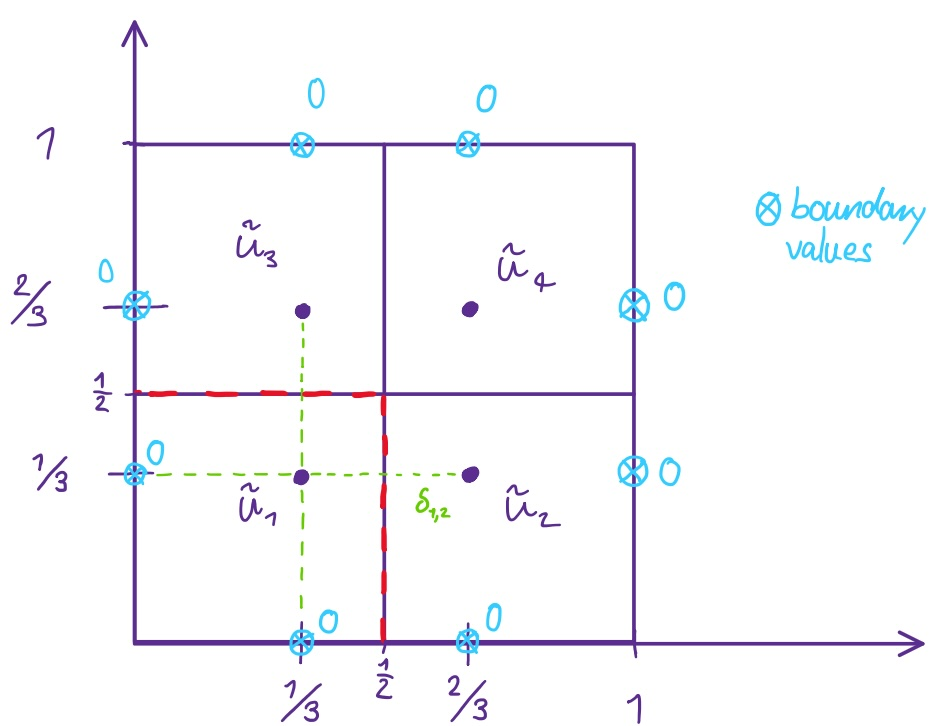
\includegraphics[width=0.8\columnwidth]{images/voronoi_example_geometry}}

\textbf{Solution}

The area of the cell is approximatively
$\int_{\Gamma_p} f(x,y)\ dxdy \approx f(P)\cdot h^2$ with cell length $h$ which is always
$\sfrac{1}{4}$ in our case. Therefore, we formulate the linear system:

For $\utild_1$:

{\color{gray}
    Caution at boundary (\faWarning):
    The dashed line usually has different length there.
    In the example, it stayed the same due to the equidistant points, but for e.g. 1/4 and 3/4 points,
    it would be 1/4 on boundary and 1/2 for inter-point distances.
}

\begin{align*}
    \frac{\utild_2 - \utild_1}{\color{green}\sfrac{1}{3}}\cdot{\color{red}\frac{1}{2}}
    + \frac{\utild_3 - \utild_1}{\color{green}\sfrac{1}{3}}{\color{red}\frac{1}{2}}
    + \frac{{\color{blue}0} - \utild_1}{\underbrace{\color{green}\sfrac{1}{3}}_\text{\faWarning}}{\color{red}\frac{1}{2}}
    + \frac{{\color{blue}0} - \utild_1}{\underbrace{\color{green}\sfrac{1}{3}}_\text{\faWarning}}{\color{red}\frac{1}{2}}
    & = \iint_{V_1} 1\ dA = \frac{1}{4} \\
    \frac{3}{2}(\utild_2 - \utild_1 + \utild_3 - \utild_1 - \utild_1 - \utild_1) & = \frac{1}{4} \\
    \utild_2 + \utild_3 - 4\utild_1 & = \frac{2}{12} = \frac{1}{6}
\end{align*}

Due to symmetry, we receive:
\begin{align*}
    \left|
    \begin{array}{llllr}
        -4\utild_1 & + \utild_2 & + \utild_3 & & = \sfrac{1}{6} \\
        \utild_1   & -4\utild_2 & & + \utild_4 & = \sfrac{1}{6} \\
        \utild_1 & & -4\utild_3 & + \utild_4 & = \sfrac{1}{6} \\
        & \utild_2 & + \utild_3 & -4\utild_4 & = \sfrac{1}{6}
    \end{array}
    \right|
\end{align*}

with $\utild = (-\sfrac{1}{12}, -\sfrac{1}{12}, -\sfrac{1}{12}, -\sfrac{1}{12})$













































